\chapter{Arhitektura i dizajn sustava}
%			\textbf{\textit{dio 1. revizije}}\\	
%			\textit{ Potrebno je opisati stil arhitekture te identificirati: podsustave, %preslikavanje na radnu platformu, spremišta podataka, mrežne protokole, globalni upravljački tok i sklopovsko-programske zahtjeve. Po točkama razraditi i popratiti odgovarajućim skicama:}
%		\begin{itemize}
%			\item 	\textit{izbor arhitekture temeljem principa oblikovanja pokazanih na predavanjima (objasniti zašto ste baš odabrali takvu arhitekturu)}
%			\item 	\textit{organizaciju sustava s najviše razine apstrakcije (npr. klijent-poslužitelj, baza podataka, datotečni sustav, grafičko sučelje)}
%			\item 	\textit{organizaciju aplikacije (npr. slojevi frontend i backend, MVC arhitektura) }		
%		\end{itemize}
	Arhitektura se može podjeliti na sljedeće sustave:
	\begin{packed_item}
		\item 	Web preglednik
		\item 	Web poslužitelj
		\item 	Baza podataka
	\end{packed_item}	

	\begin{figure}[H]
		\centering
		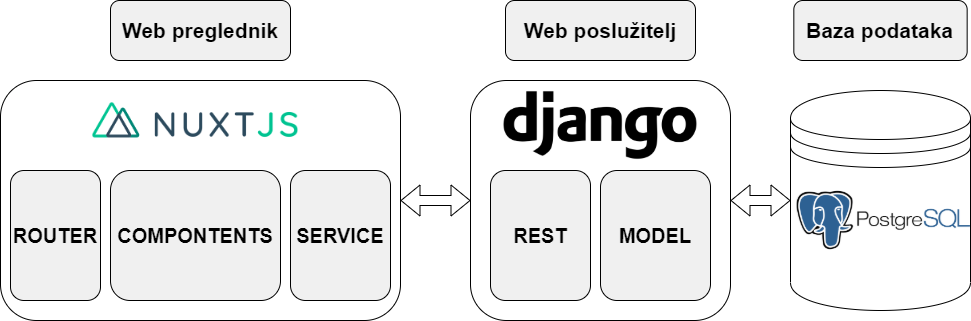
\includegraphics[scale=0.45]{slike/ARHITEKTURA.PNG}
		\caption{Arhitektura sustava}
		\label{fig:promjene}
	\end{figure}	

	\underline{\textit{Web preglednik}} je program čije je svrha omogućiti pregled web-stranice te njenog multimedijalnog sadržaja. Osim samog pregleda, web preglednik mora moći prevesti kôd stoga jer je on ujedno i kompajler. U našem slučaju web preglednik će prevoditi kôd radnog okvira (\emph{engl. framework}) Nuxt.js koje je proširenje Vue.js frameworka.

	\underline{\textit{Web poslužitelj}} je sustav koji treba omogućiti odvijanje komunikacije web preglednika i baze podataka. Njegova zadaća je obrađivati zahtjeve koje zahtjeva web preglednik, po potrebi komunicirati s bazom podataka te vratiti rezultat obrade. Rezultat obrade biti se će SSR (engl. Server Side Rendered) - statički generirana stranica. Komunikacija s poslužiteljem odvija se putem protokola HTTP (\emph{engl. Hyper Text Transfer Protocol}). U našem slučaju za izradu web poslužitelja koristimo Python framework Django koji je besplatan i \emph{open source}.

	\underline{\textit{Baza podataka}} je sustav za trajnu pohranu podataka. U našem slučaju koristimo relacijsku bazu podataka PostgreSQL.

	Zadana arhitektura temelji se na prikazu statički generirane stranice dobivene s web poslužitelja (Django servera). Prema zahtjevu web klijenta Nuxt.js generira zahtjev na API web poslužitelja te dobiva odgovor u obliku generirane statičke stranice. Web poslužitelj prema potrebi šalje zahtjev za dohvat podataka iz baze podataka kako bi mogao stranicu popuniti s relevantnim podacima i multimedijom.

	Django nije tradicionalni MVC (Model-View-Controller) framework, ali se ponaša vrlo slično MVC koncept modelu. MVC koncept model sastoji se od sljedećih komponenata: 
	\begin{packed_item}
		\item{\underline{\textit{Model}} - Dinamičke strukture podataka koje se popunjavaju iz baze podatka za svrhu prikaza ili se popunjavaju iz korisničkog sučelja u svrhu pohrane.}
		\item{\underline{\textit{View}} - Korisničko sučelje preko kojega korisnik podatke prenosi u Model.}
		\item{\underline{\textit{Controller}} - Sučelje između Modela i View-a. Manipulira podacima kako bi ih Model mogao obraditi ili manipulira podatke da ih View može prikazati.}
	\end{packed_item}

	Django razvojni tim preferira koristi koncept MTV (\emph{Model-Template-View}) modela. Razlika između MVC modela i MTV modela je što se komponenta View naziva Template, a komponenta Controller se naziva View.

	\pagebreak
				
	\section{Baza podataka}
		
		\begin{comment}
			\textbf{\textit{dio 1. revizije}}\\
			
		\textit{Potrebno je opisati koju vrstu i implementaciju baze podataka ste odabrali, glavne komponente od kojih se sastoji i slično.}
		\end{comment}
				
		\noindent Za potrebe našeg sustava koristit ćemo relacijsku bazu podataka PostgreSQL.
		Baza se sastoji od relacija (tablica) i njihovih atributa. Bazu podataka koristimo za pohranu informacija o korisnicima, njihovim rezervacijama i podacima o praonici.
		Baza podataka ove aplikacije sastoji se od sljedećih entiteta:
		\begin{packed_item}
			\item 	Machine
			\item 	Appointment
			\item 	User
			\item 	Post
			\item 	Recension
			\item 	Washday
		\end{packed_item}	
	
		\noindent Osim naših tablica, Django sam stvara nove tablice poput permissiona, sessiona i logova.
		
			\subsection{Opis tablica}
			
				\begin{comment}
				\textit{Svaku tablicu je potrebno opisati po zadanom predlošku. Lijevo se nalazi točno ime varijable u bazi podataka, u sredini se nalazi tip podataka, a desno se nalazi opis varijable. Svjetlozelenom bojom označite primarni ključ. Svjetlo plavom označite strani ključ}
				
				\begin{longtabu} to \textwidth {|X[6, l]|X[6, l]|X[20, l]|}
					
					\hline \multicolumn{3}{|c|}{\textbf{korisnik - ime tablice}}	 \\[3pt] \hline
					\endfirsthead
					
					\hline \multicolumn{3}{|c|}{\textbf{korisnik - ime tablice}}	 \\[3pt] \hline
					\endhead
					
					\hline 
					\endlastfoot
					
					\cellcolor{LightGreen}IDKorisnik & INT	&  	Lorem ipsum dolor sit amet, consectetur adipiscing elit, sed do eiusmod tempor incididunt ut labore et dolore magna aliqua. Ut enim ad minim veniam 	\\ \hline
					korisnickoIme	& VARCHAR &   	\\ \hline 
					email & VARCHAR &   \\ \hline 
					ime & VARCHAR	&  		\\ \hline 
					\cellcolor{LightBlue} primjer	& VARCHAR &   	\\ \hline 
					
					
				\end{longtabu}
				\end{comment}
			
			\noindent\textbf{Machine}  Ovaj entitet sadrži sve važne informacije vezane za uređaj u praonici. Sadrži atribute: id uređaja i type. Ovaj entitet u vezi je \textit{Many-to-One} s entitetom Appointment preko id-a uređaja.
			
			\begin{longtabu} to \textwidth {|X[8, l]|X[6, l]|X[20, l]|}
				
				\hline \multicolumn{3}{|c|}{\textbf{Machine}}	 \\[3pt] \hline
				\endfirsthead
				
				\hline \multicolumn{3}{|c|}{\textbf{Machine}}	 \\[3pt] \hline
				\endhead
				
				\hline 
				\endlastfoot
				
				\textbf{id} & INT	&  jedinstveni brojčani identifikator	\\ \hline
				type & BOOLEAN &  vrsta uređaja (perilica ili sušilica)\\ \hline 
				
				
			\end{longtabu}
		
			\noindent\textbf{Appointment}  Ovaj entitet sadrži sve važne informacije vezane za rezervirani termin u praonici. Sadrži atribute: id termina, time, machine\_id, price, opcionalni note, paid, basket\_taken, user\_id i employee\_id. Ovaj entitet u vezi je \textit{One-to-Many} s entitetom Machine preko id-a uređaja, vezi \textit{Many-to-One} s entitetom User preko id-a korisnika i id-a zaposlenika.
		
			\begin{longtabu} to \textwidth {|X[8, l]|X[6, l]|X[20, l]|}
				
				\hline \multicolumn{3}{|c|}{\textbf{Appointment}}	 \\[3pt] \hline
				\endfirsthead
				
				\hline \multicolumn{3}{|c|}{\textbf{Appointment}}	 \\[3pt] \hline
				\endhead
				
				\hline 
				\endlastfoot
				\textbf{id} & INT	&  jedinstveni brojčani identifikator	\\ \hline
				time & TIMESTAMP	&  	datum rezerviranog termina u praonici i vrijeme početka 	\\ \hline
				machine\_id (FK)	& INT &  jedinstveni identifikator uređaja kojeg rezerviramo u terminu (machine.id) 	\\ \hline 
				price & FLOAT &  cijena usluge koju korisnik plaća (pranje ili sušenje) \\ \hline 
				note & VARCHAR	& opcionalna bilješka zaposleniku \\ \hline 
				paid & BOOLEAN	& korisnik bira hoće li platiti termin online ili uživo	\\ \hline 
				basket\_taken & BOOLEAN	& korisnik može posuditi jednu košaru iz praonice 	\\ \hline 
				user\_id (FK)	& INT &  jedinstveni identifikator korisnika koji je rezervirao termin (user.id) 	\\ \hline 
				employee\_id (FK)	& INT &  jedinstveni identifikator zaposlenika koji radi za vrijeme rezerviranog termina (user.id)	\\ \hline
				
			\end{longtabu}
		
			\noindent\textbf{User}  Ovaj entitet sadrži sve važne informacije vezane za različite korisnike u praonici. Sadrži atribute: id korisnika, username, password, first\_name, last\_name, jedinstveni JMBAG, jedinstveni email, is\_active, is\_staff, card\_number, negative\_points, date\_joined, last\_login, is\_superuser. Ovaj entitet u vezi je \textit{One-to-Many}  \textit{One-to-Many} s entitetom Appointment preko id-a korisnika, u vezi \textit{One-to-Many} s entitetom Post preko id-a korisnika i u vezi \textit{One-to-Many} s entitetom Recension preko id-a korisnika.
		
			\begin{longtabu} to \textwidth {|X[8, l]|X[6, l]|X[20, l]|}
				
				\hline \multicolumn{3}{|c|}{\textbf{User}}	 \\[3pt] \hline
				\endfirsthead
				
				\hline \multicolumn{3}{|c|}{\textbf{User}}	 \\[3pt] \hline
				\endhead
				
				\hline 
				\endlastfoot
				
				\textbf{id} & INT	&  jedinstveni brojčani identifikator korisnika	\\ \hline
				username	& VARCHAR &   korisničko ime	\\ \hline
				password	& VARCHAR &   lozinka korisničkog računa	\\ \hline
				first\_name	& VARCHAR &   ime korisnika	\\ \hline 
				last\_name	& VARCHAR &   prezime korisnika	\\ \hline
				JMBAG	& VARCHAR &   JMBAG korisnika	\\ \hline
				email	& VARCHAR &   jedinstveni email korisnika	\\ \hline
				is\_active & BOOLEAN &  svi korisnici čije registracije su potvrđene od zaposlenika i koji nisu blokirani\\ \hline 
				is\_staff & BOOLEAN &  oznaka je li korisnik i zaposlenik\\ \hline 
				is\_superuser	& BOOLEAN &   pokazuje je li korisnik ujedno i administrator	\\ \hline
				card\_number	& VARCHAR &   broj kreditne kartice korisnika	\\ \hline
				negative\_points	& INT &   broj negativnih bodova korisnika	\\ \hline
				date\_joined	& DATE &   datum registracije korisnika	\\ \hline
				last\_login	& TIMESTAMP &  vrijeme zadnje prijave u sustav	\\ \hline
			
				
				
			\end{longtabu}
		
			\noindent\textbf{Post}  Ovaj entitet sadrži sve važne informacije vezane za objavu. Sadrži atribute: id objave, photo, text, date, type i employee\_id. 
			Ovaj entitet u vezi je \textit{Many-to-One} s entitetom User preko id-a zaposlenika.
		
			\begin{longtabu} to \textwidth {|X[8, l]|X[6, l]|X[20, l]|}
				
				\hline \multicolumn{3}{|c|}{\textbf{Post}}	 \\[3pt] \hline
				\endfirsthead
				
				\hline \multicolumn{3}{|c|}{\textbf{Post}}	 \\[3pt] \hline
				\endhead
				
				\hline 
				\endlastfoot
				
				\textbf{id} & INT	&  jedinstveni brojčani identifikator objave	\\ \hline
				photo	& BYTEA &   opcionalna slika priložena uz objavu	\\ \hline 
				text	& VARCHAR &   tekst objave	\\ \hline
				date	& DATE &  datum objavljivanja objave	\\ \hline
				type	& BOOLEAN &   ako je vrijednost zastavice 1, objava se prikazuje na "LostAndFound" stranici 	\\ \hline
				employee\_id (FK)	& INT &  id zaposlenika koji radi za vrijeme rezerviranog termina (user.id) 	\\ \hline		
						
				
				
			\end{longtabu}
		
			\noindent\textbf{Recension}  Ovaj entitet sadrži sve važne informacije vezane za recenzije. Sadrži atribute: id recenzije, user\_id, employee\_id, text i grade. Ovaj entitet u vezi je \textit{Many-to-One} s entitetom User preko id-a zaposlenika i id-a korisnika.
		
			\begin{longtabu} to \textwidth {|X[8, l]|X[6, l]|X[20, l]|}
				
				\hline \multicolumn{3}{|c|}{\textbf{Recension}}	 \\[3pt] \hline
				\endfirsthead
				
				\hline \multicolumn{3}{|c|}{\textbf{Recension}}	 \\[3pt] \hline
				\endhead
				
				\hline 
				\endlastfoot
				
				\textbf{id} & INT	&  jedinstveni brojčani identifikator recenzije	\\ \hline
				user\_id (FK)	& INT &  id korisnika koji je ostavio recenziju (user.id) 	\\ \hline
				employee\_id (FK)	& INT &  id recenziranog zaposlenika (user.id)	\\ \hline
				text	& VARCHAR &   tekst recenzije	\\ \hline
				grade	& INT & ocjena zaposlenika od 1 do 5	\\ \hline
				
			\end{longtabu}
			
			\noindent\textbf{Washday}  Ovaj entitet sadrži sve važne informacije vezane za radni dan praonice. Sadrži atribute: id radnog dana, date, open\_time, close\_time, pause\_start, pause\_end i wash\_price. Ovaj entitet nije u vezi ni s jednim drugim entitetom.
			
			\begin{longtabu} to \textwidth {|X[8, l]|X[6, l]|X[20, l]|}
				
				\hline \multicolumn{3}{|c|}{\textbf{Washday}}	 \\[3pt] \hline
				\endfirsthead
				
				\hline \multicolumn{3}{|c|}{\textbf{Washday}}	 \\[3pt] \hline
				\endhead
				
				\hline 
				\endlastfoot
				
				\textbf{id} & INT	&  jedinstveni brojčani  identifikator radnog dana praonice	\\ \hline
				date & DATE	&  trenutni datum	\\ \hline
				open\_time	& TIME &   početak radnog vremena	\\ \hline
				close\_time	& TIME & kraj radnog vremena	\\ \hline
				pause\_start	& TIME & početak pauze	\\ \hline
				pause\_end	& TIME & kraj pauze	\\ \hline
				wash\_price	& FLOAT & cijena jednog pranja	\\ \hline
				drying\_price	& FLOAT & cijena jednog sušenja	\\ \hline
				
				
			\end{longtabu}
			
			
			\subsection{Dijagram baze podataka}
			\begin{comment}
				\textit{ U ovom potpoglavlju potrebno je umetnuti dijagram baze podataka. Primarni i strani ključevi moraju biti označeni, a tablice povezane. Bazu podataka je potrebno normalizirati. Podsjetite se kolegija "Baze podataka".}
			\end{comment}
				
				\begin{figure}[H]
					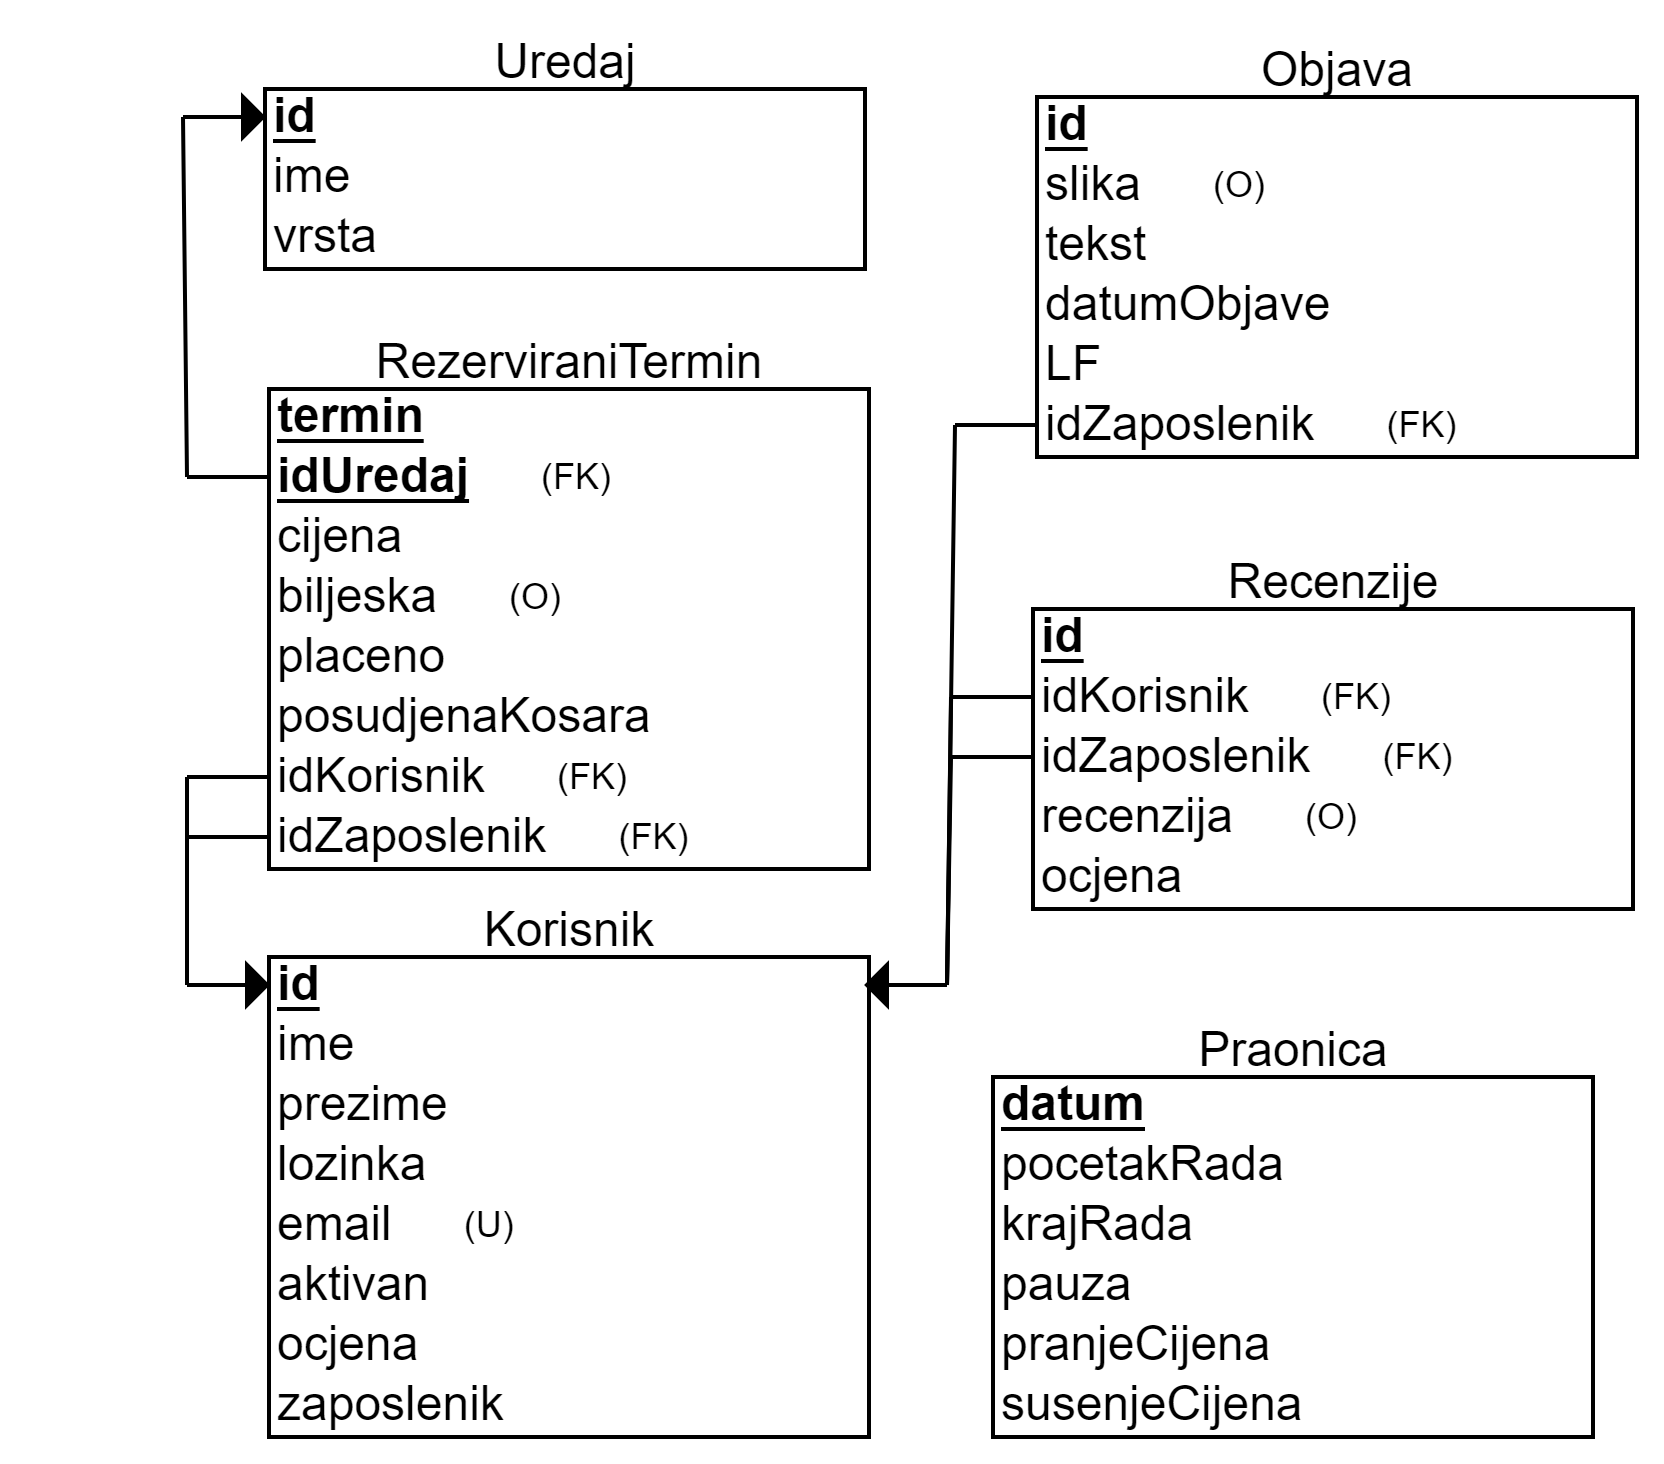
\includegraphics[scale=0.2]{slike/BAZA.PNG} %veličina slike u odnosu na originalnu datoteku i pozicija slike
					\centering
					\caption{Relacijska shema baze podataka}
					\label{fig:promjene}
				\end{figure}
			\eject
			
			
			\begin{figure}[H]
				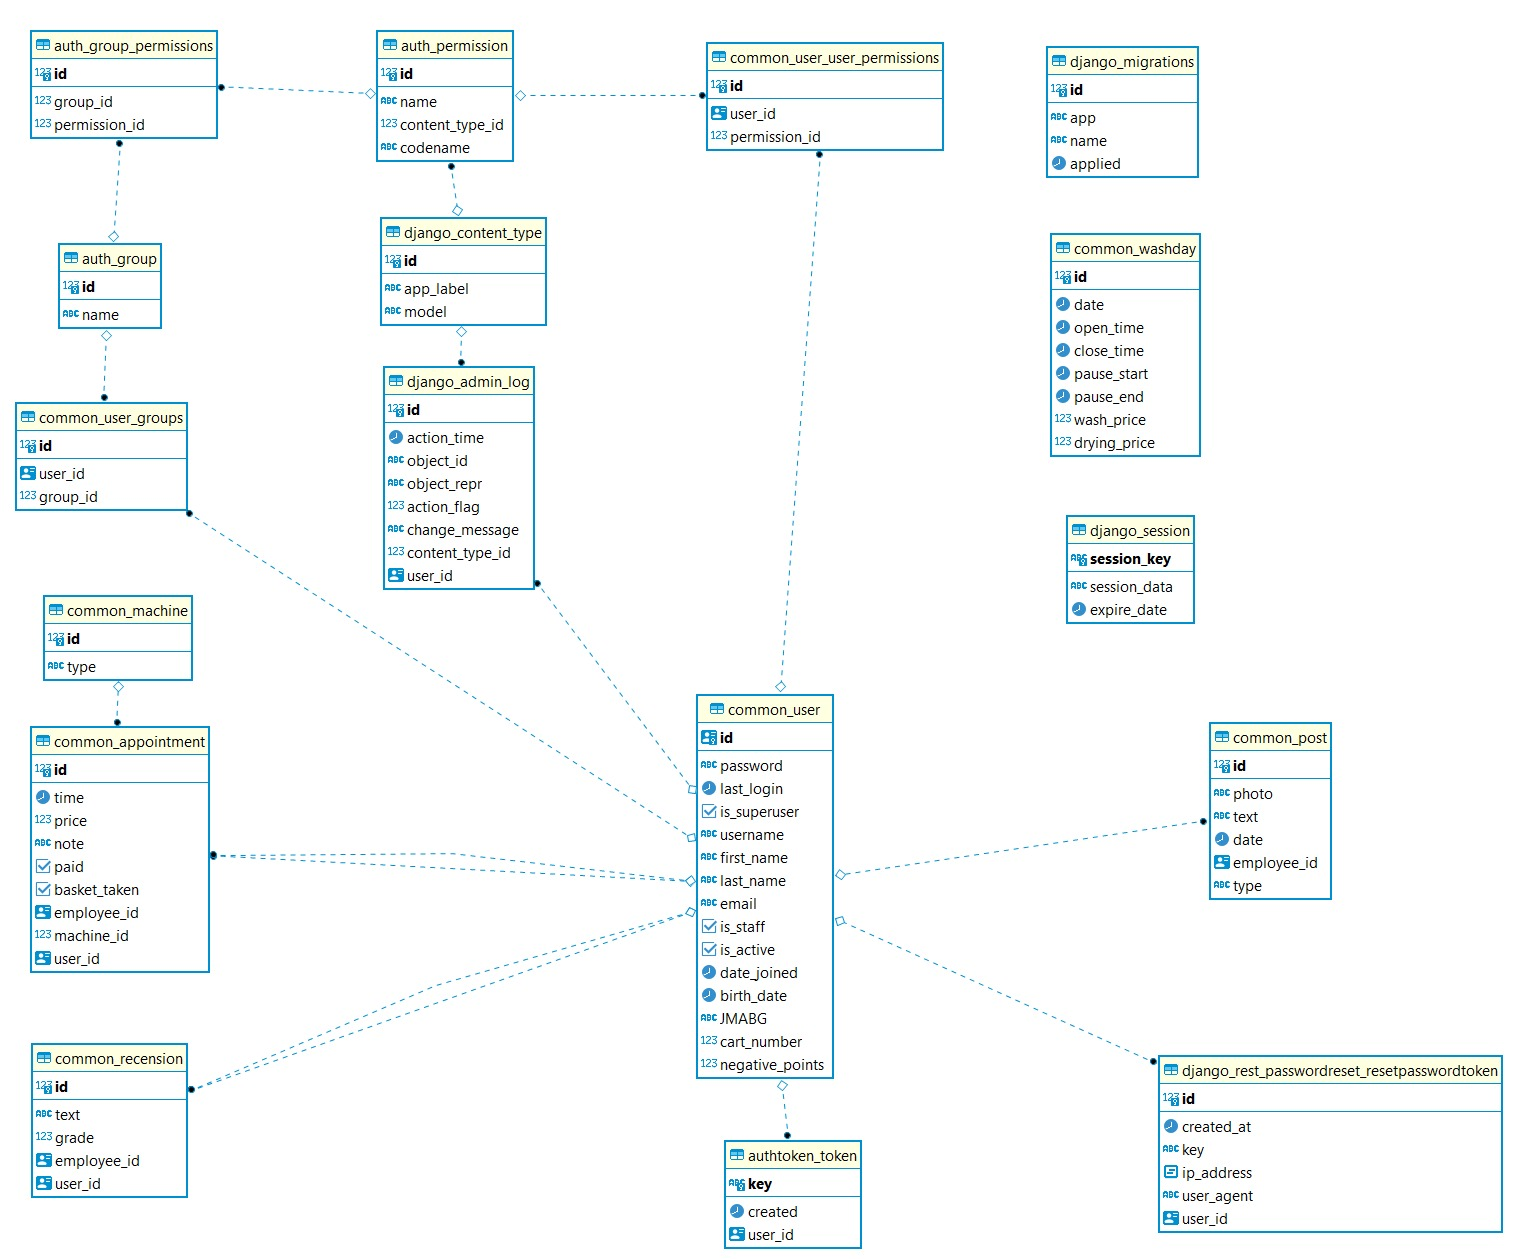
\includegraphics[scale=0.3]{slike/djangoBaza.jpeg} %veličina slike u odnosu na originalnu datoteku i pozicija slike
				\centering
				\caption{Relacijska shema Django baze podataka}
				\label{fig:promjene}
			\end{figure}
			\eject
			
			
		\section{Dijagram razreda}
		\begin{comment}
			\textit{Potrebno je priložiti dijagram razreda s pripadajućim opisom. Zbog preglednosti je moguće dijagram razlomiti na više njih, ali moraju biti grupirani prema sličnim razinama apstrakcije i srodnim funkcionalnostima.}\\
			
			\textbf{\textit{dio 1. revizije}}\\
			
			\textit{Prilikom prve predaje projekta, potrebno je priložiti potpuno razrađen dijagram razreda vezan uz \textbf{generičku funkcionalnost} sustava. Ostale funkcionalnosti trebaju biti idejno razrađene u dijagramu sa sljedećim komponentama: nazivi razreda, nazivi metoda i vrste pristupa metodama (npr. javni, zaštićeni), nazivi atributa razreda, veze i odnosi između razreda.}\\
			
			\textbf{\textit{dio 2. revizije}}\\			
			
			\textit{Prilikom druge predaje projekta dijagram razreda i opisi moraju odgovarati stvarnom stanju implementacije} \\
		\end{comment}
			
			Zbog toga što je web poslužitelj napisan u Pythonu, ne možemo reći da u našem web modelu postoje razredi u pravom smislu riječi. Naime, moguće je pisati razred u Pythonu, ali nije moguće koristiti vrste pristupa. Sve metode, razredi i atributi su javne (i tako će biti označene na dijagramima). Moguće je naznačiti da želimo da se komponenta ponaša kao privatna korištenjem donje crtice u njenom imenu. Stoga zaključujemo da razredi u Pythonu postoje i moguće je izraditi dijagram razreda za komponente web aplikacije iako razredi nemaju potpune funkcionalnosti objektno orijentiranog jezika. Django koristi razrede prilikom svoje implementacije. Kao što je već navedeno, Django se temelji na modelu MTV (\emph{Model-Template-View}).\\\
			
			\pagebreak
			\emph{Models} u Djangu su Python razredi koji se automatski prenose u obliku relacija u bazu podataka korištenjem Djangovih karakterističnih \emph {migrate} funkcionalnosti.  Prilikom pisanja Modela potrebno je obratiti pozornost na njihovu povezanost i buduću brojnost u bazi podataka. 	
			\begin{figure}[H]
				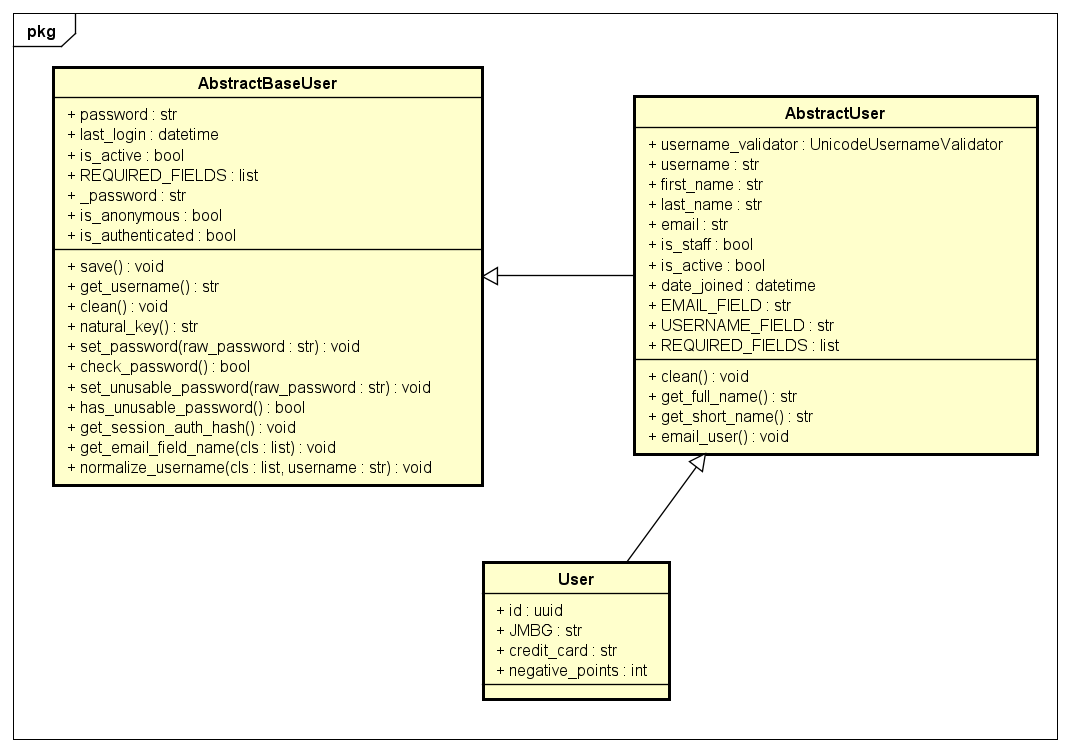
\includegraphics[scale=0.55]{slike/Razredni_dijagrami_Models.PNG} 
				\centering
				\caption{Dijagram razreda - dio Models}
				\label{fig:promjene}
			\end{figure}
		
			\pagebreak
			\emph{Views} sadrže svu funkcionalnost i strukture podataka potrebne da se povežu funkcionalnosti Templatea i Modela. Osim što povezuju ta dva dijela sustava, views mogu sadržavati dodatnu funkcionalnost.
			\begin{figure}[H]
				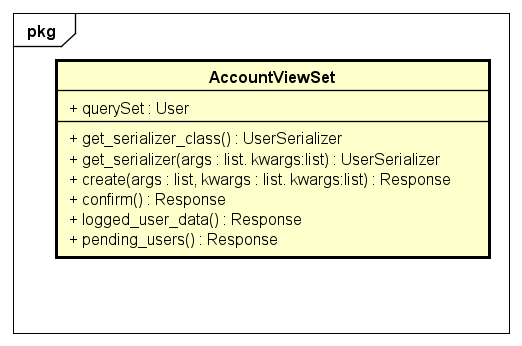
\includegraphics[scale=0.55]{slike/Razredni_dijagrami_Views.PNG}
				\centering
				\caption{Dijagram razreda - dio Views}
				\label{fig:promjene}
			\end{figure}  	
		
		 	\pagebreak			
 			\emph{Templates} sadrže sve strukture podataka potrebne da se podatak prenese s korisničkog sučelja u model. U našem slučaju korisničko sučelje dio je Nuxt.js radnog okvira. Nuxt.js uz pomoć \emph{axios} sustava prenosi podatke na View.
 			\begin{figure}[H]
 				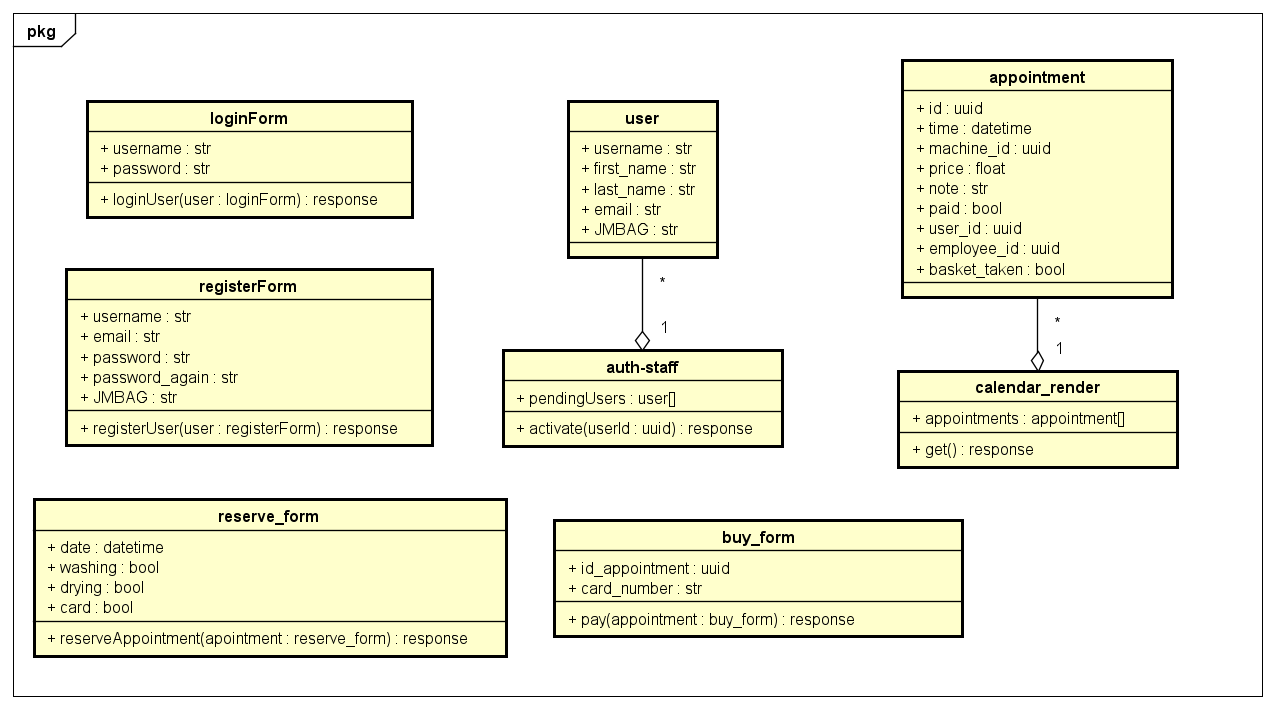
\includegraphics[scale=0.45]{slike/Razredni_dijagrami_Templates.PNG}
 				\centering
 				\caption{Dijagram razreda - dio Templates}
 				\label{fig:promjene}
 			\end{figure} 	
 		
			\pagebreak
 			
 			
		\section{Dijagram stanja}
			
			
			\textbf{\textit{dio 2. revizije}}\\
			
			\textit{Potrebno je priložiti dijagram stanja i opisati ga. Dovoljan je jedan dijagram stanja koji prikazuje \textbf{značajan dio funkcionalnosti} sustava. Na primjer, stanja korisničkog sučelja i tijek korištenja neke ključne funkcionalnosti jesu značajan dio sustava, a registracija i prijava nisu. }
			
			
			\eject 
		
		\section{Dijagram aktivnosti}
		
		Dijagram aktivnosti primjenjuje se za opis modela toka upravljanja ili toka podataka. Ne upotrebljava se za modeliranje događajima poticanog ponašanja. U modeliranju toka upravljanja svaki novi korak poduzima se nakon završenog prethodnog, a naglasak je na jednostavnosti. Na dijagramu aktivnosti 4.7 prikazan je
		proces rezervacije termina u praonici. Korisnik se prijavi u sustav, odabire stranicu Rezervacije koja prikaže kalendar s dostupnim terminima za rezervaciju i odabire slobodan termin. Zatim mu se prikazuje forma preko koje može odabrati posudbu košare te napisati bilješku. Nakon toga odabire Rezerviraj čime se termin rezervira te se korisniku prikaže osvježen kalendar s njegovom upisanom rezervacijom termina.

		
				\begin{figure}[H]
				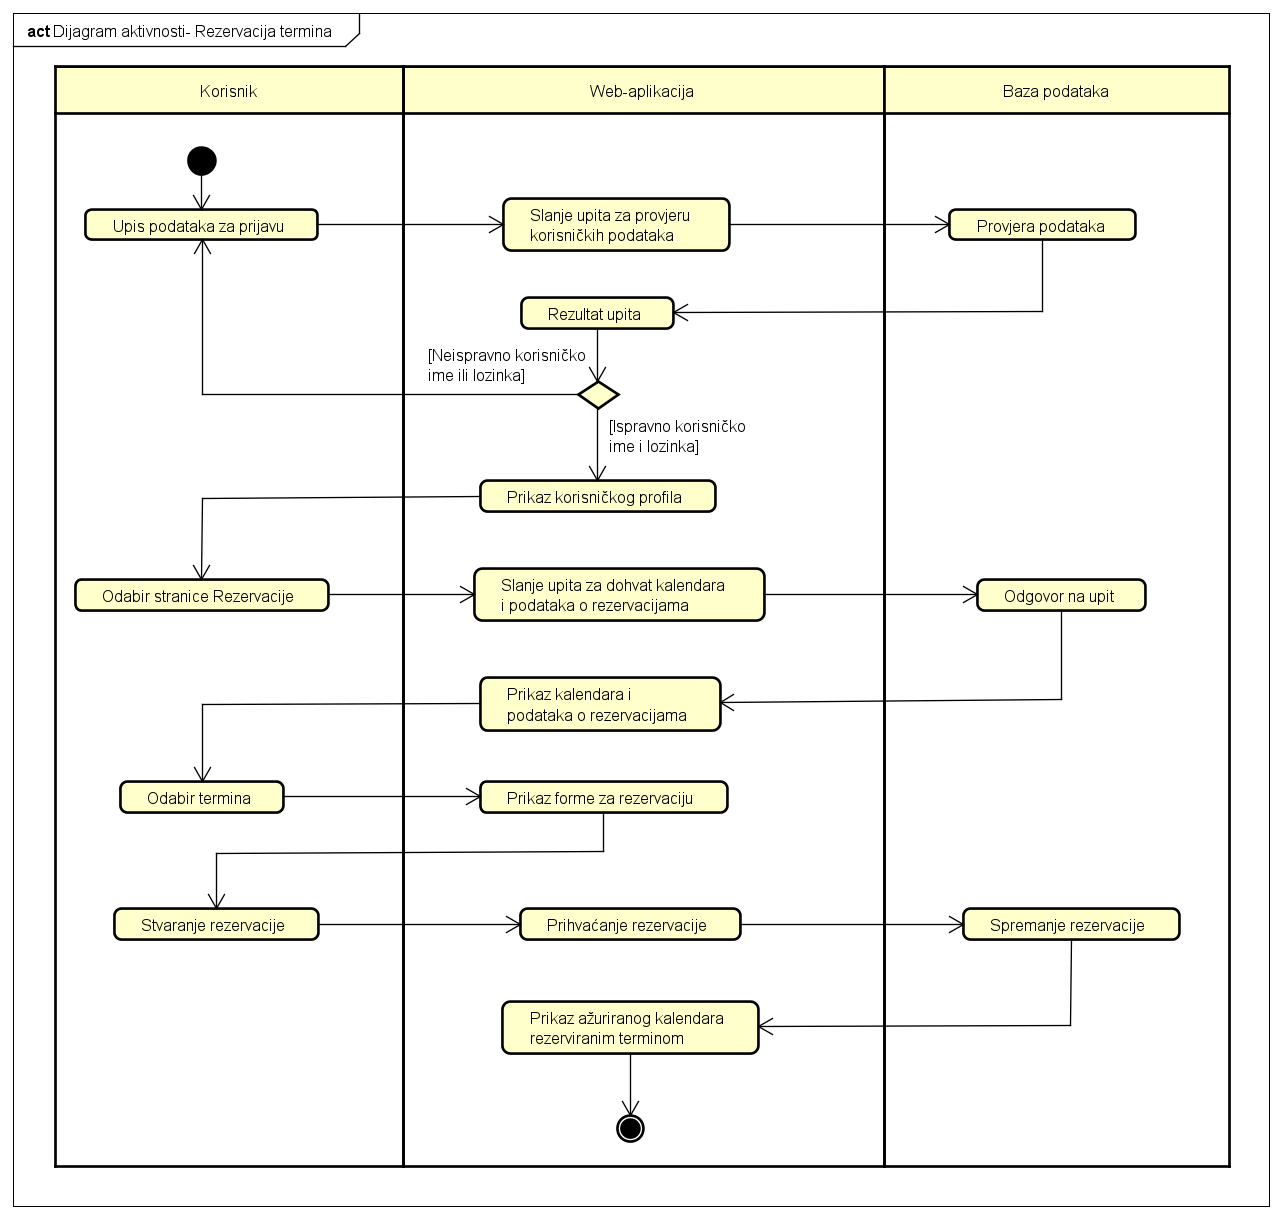
\includegraphics[width=1\linewidth]{slike/Dijagram aktivnosti.png}
				\centering
				\caption{Dijagram aktivnosti}
				\label{fig:promjene}
			\end{figure}
			\eject
		\section{Dijagram komponenti}
		
			Dijagram komponenti prikazan slikom 4.7 prikazuje komponente i njihovu ovisnost unutar aplikacije. \\Nuxt ima funkciju routera koji u ovisnosti o url-u na frontend web aplikacije šalje odgovarajuće HTML, CSS i Javascript dokumente. Sami frontend je podijeljen na logičke komponente koje su nazvane ovisno o imenu stranice tj. dijelu aplikacije kojemu se pristupa. Sve frontend komponente ovisne su o \textit{layouts} i \textit{components} komponentama iz kojih povlače podatke o zaglavlju stranice koje je vidljivo u svakom trenutku.\\ Django REST API komunicira s bazom podataka te poslužuje potrebne JSON podatke koji su mu dostupni unutar baze.
			
			\begin{figure}[H]
				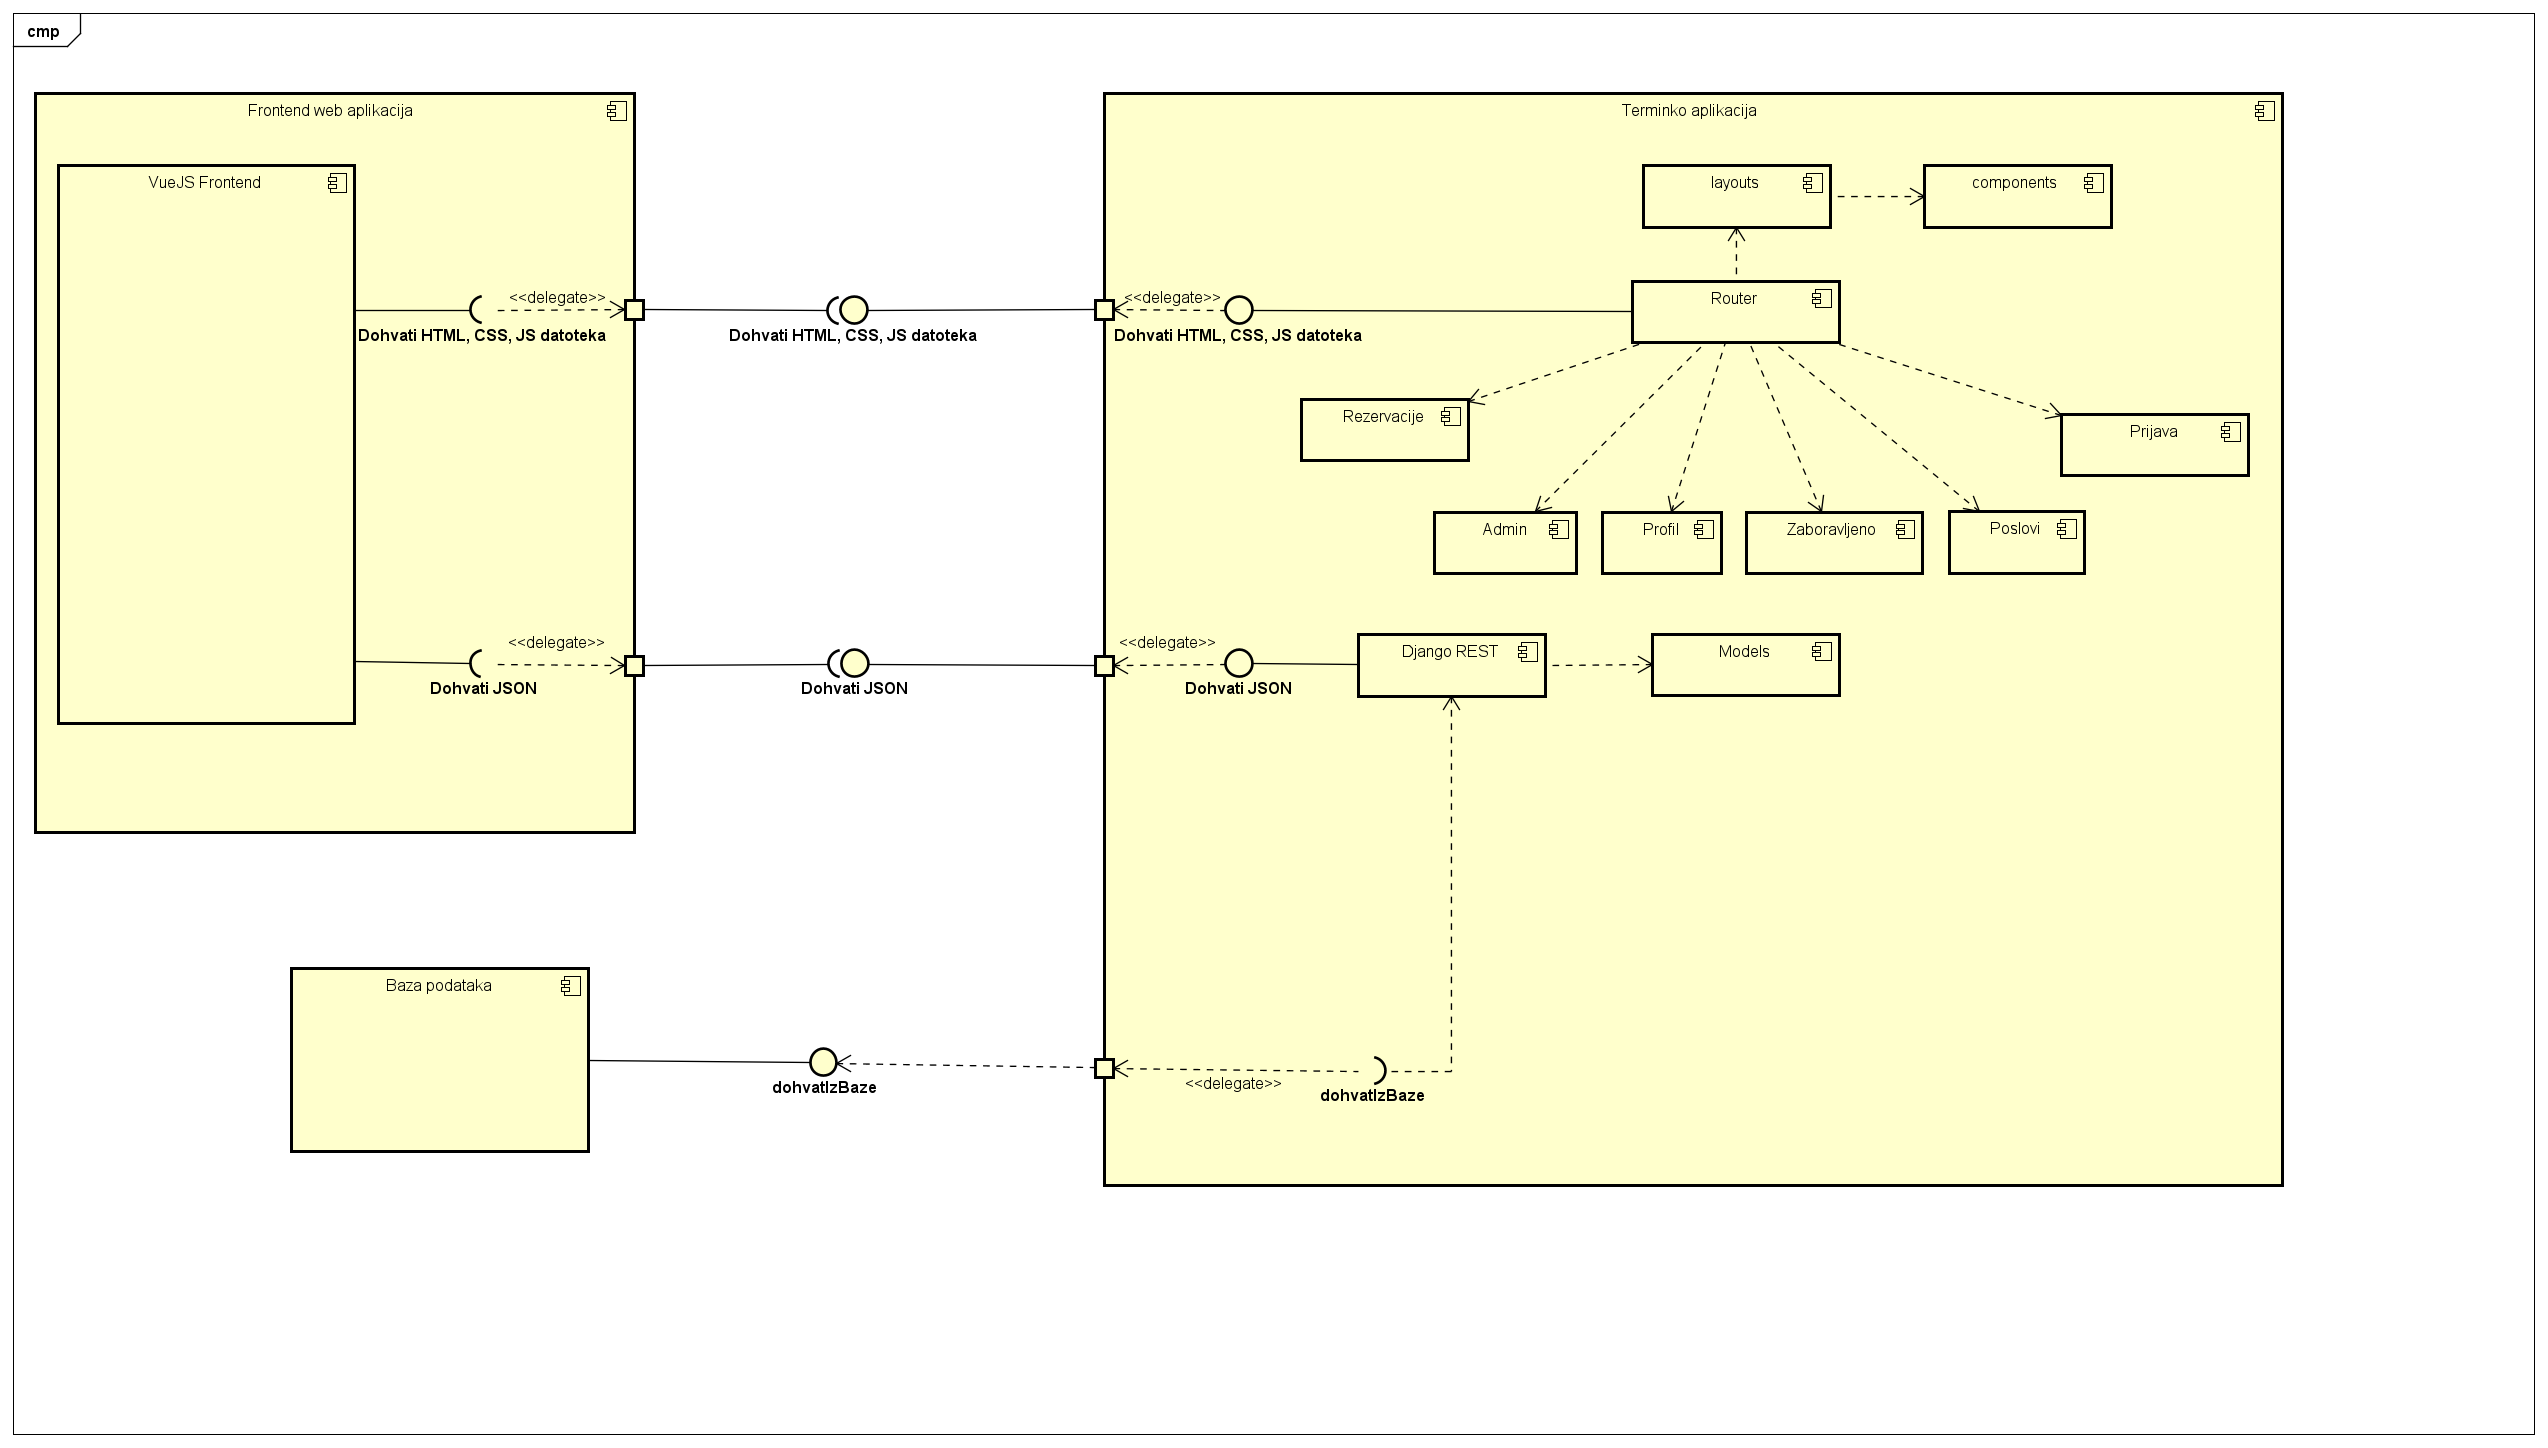
\includegraphics[width=.9\linewidth]{slike/dijagram_komponenti.PNG}
				\centering
				\caption{Dijagram komponenti}
				\label{fig:dijagram_komponenti}
			\end{figure}